% The original template (from Trevor) had a custom \appendix command,
% but I found it to break figure/table counters. I'm not sure how
% reliable my fix is, so I ended up reverting back to the standard
% latex version, and renaming the custom command to \myappendix.  You
% can try both and see how things work out:
% 1) Call \appendix once, and then make each appendix a \chapter
% 2) Call \myappendix once, and then make each appendix a \section.

\appendix
\chapter{Appendix Title}



\section{Detailed System Design of Perpendicular station}


We have developed one of the most sensitive Spin-torque ferromagnetic resonance perpendicular magnetic stations. Here we describe the detailed system designs.


\begin{figure*}[t]
  \centering
  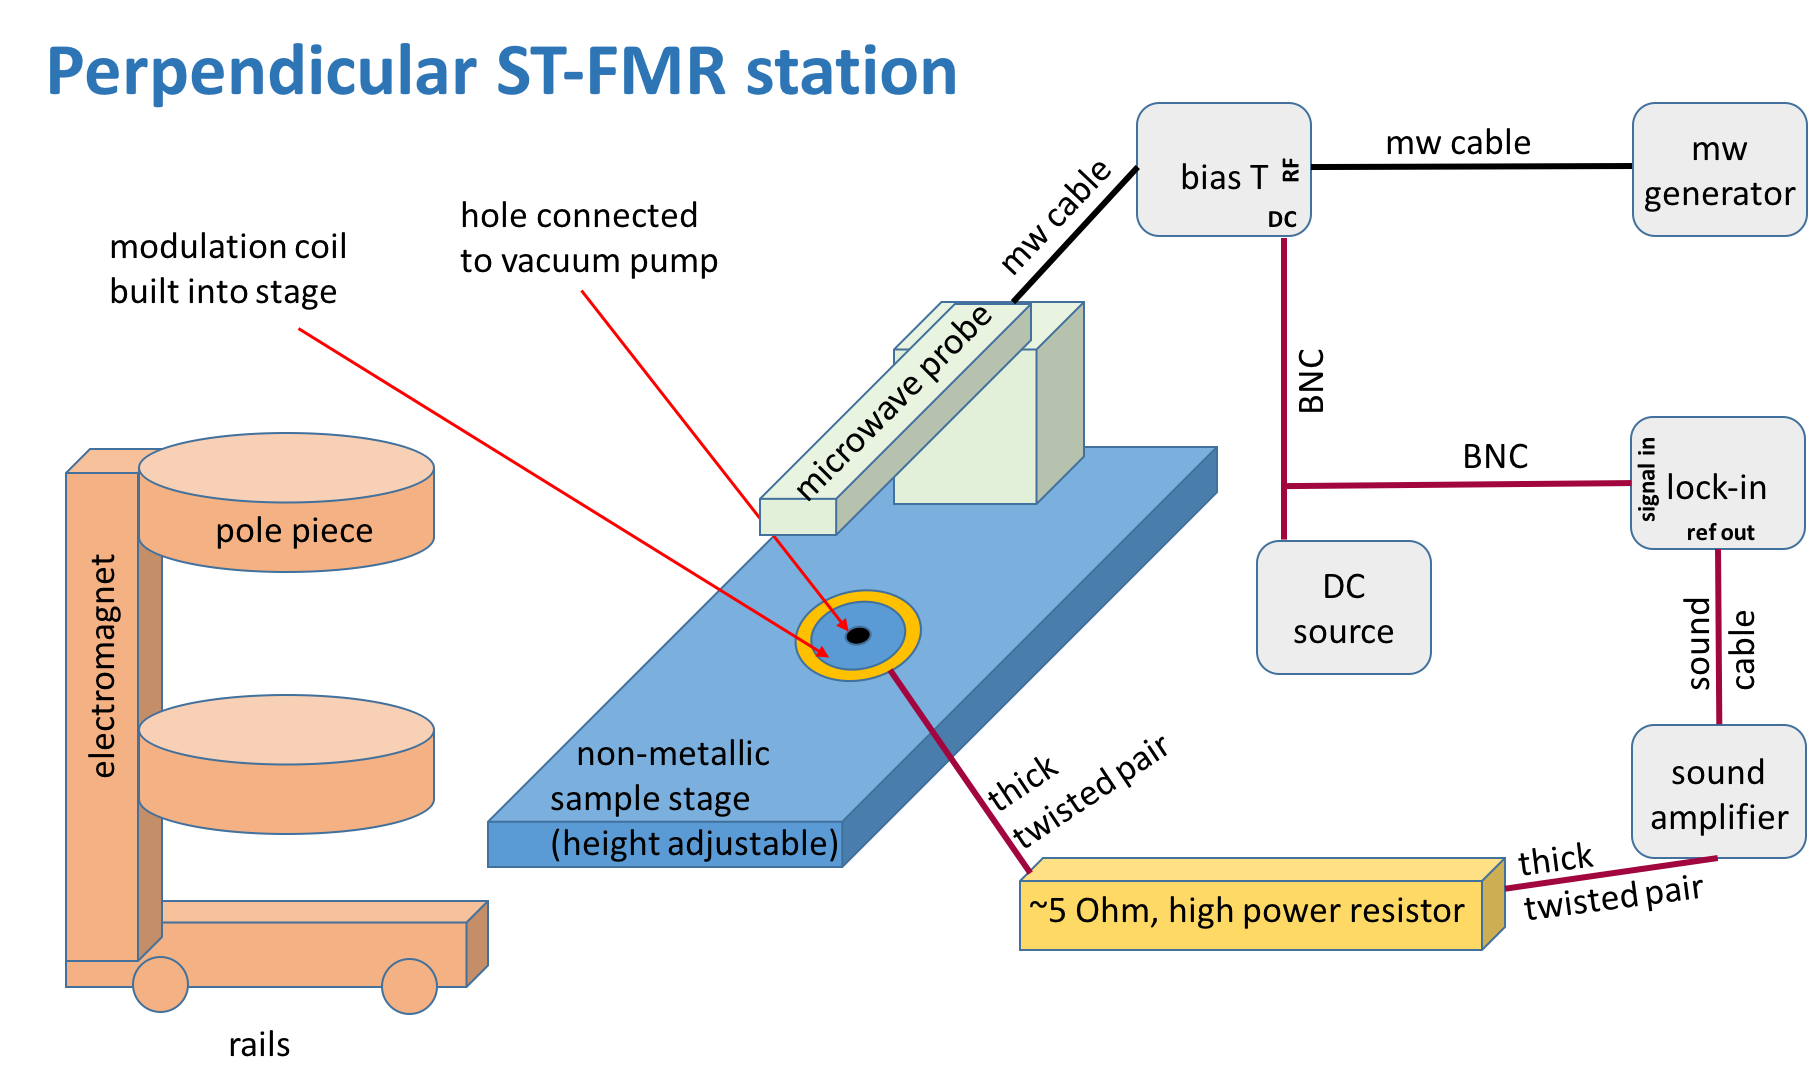
\includegraphics[width=1.0\textwidth]{fig/appendix/setup.png}
  \caption{Perpendicular ST-FMR station Setup}
  \label{fig:stationsetup}
\end{figure*}



First of all, here is all the equipments needed to build the out-of-plane magnetic probe station:

\begin{enumerate}
  \item GMW Dipole Electromagnet Model 3470
  \item Kepco bipolar operational power supply model Model 50-8M 
  \item Cascade RF probe : SG-120um
  \item Cascade RPP210-AI probe positioner (both the probe and the positioner are non-magnetic)
  \item Sentech Output 720p Cased Camera
  \item Navitar 12X Zoom Lens System
  \item AmScope LED-80M 80-LED Microscope Ring Light
\end{enumerate}

Fig.\ref{fig:stationsetup} sketches the design of the out-of-plane station.The magnet is fixed vertically on metal frame and the stage height is adjustable. At first, we can land the probe to make contact of the sample with the magnet moving away(shown in Fig.\ref{fig:operation1}. After making contact of the sample, first remove the camera (the setup could be improved by making a stationary camera). Then we can slide in the magnet so that the sample is located in the center of the magnet. It is important not to touch the probe and microwave cable when sliding the magnet. After moving the magnet we are ready to make ST-FMR measurement as showing in Fig.\ref{fig:operation2}.


\begin{figure}[!ht]
\centering
\subfigure{\label{fig:operation1}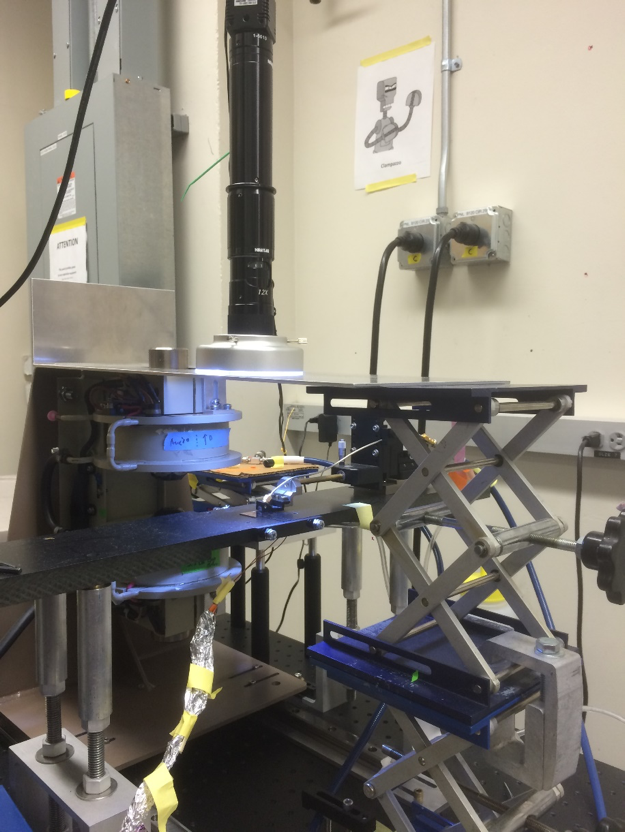
\includegraphics[width=75mm]{fig/appendix/1.png}}
\subfigure{\label{fig:operation2}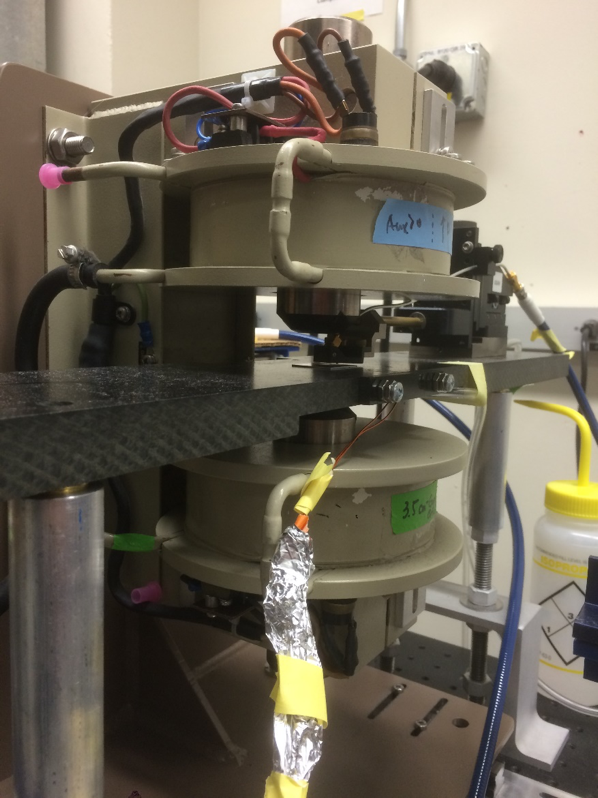
\includegraphics[width=75mm]{fig/appendix/2.png}}
\caption{Operation of Out-of-plane probe station}
\end{figure}


\begin{figure}[!ht]
\centering
\subfigure{\label{fig:operation3}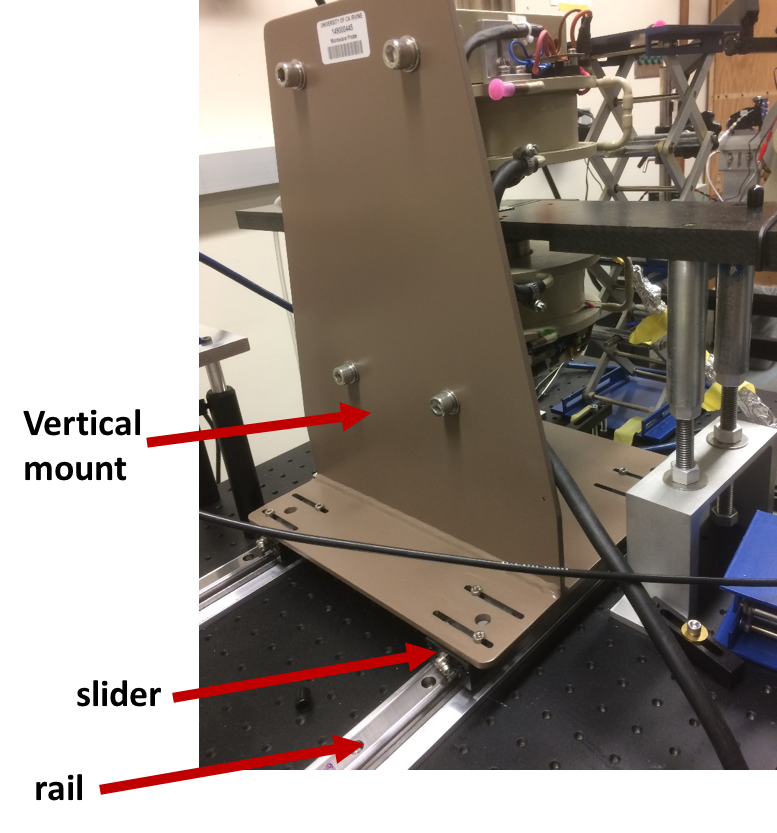
\includegraphics[width=75mm]{fig/appendix/3.png}}
\subfigure{\label{fig:operation4}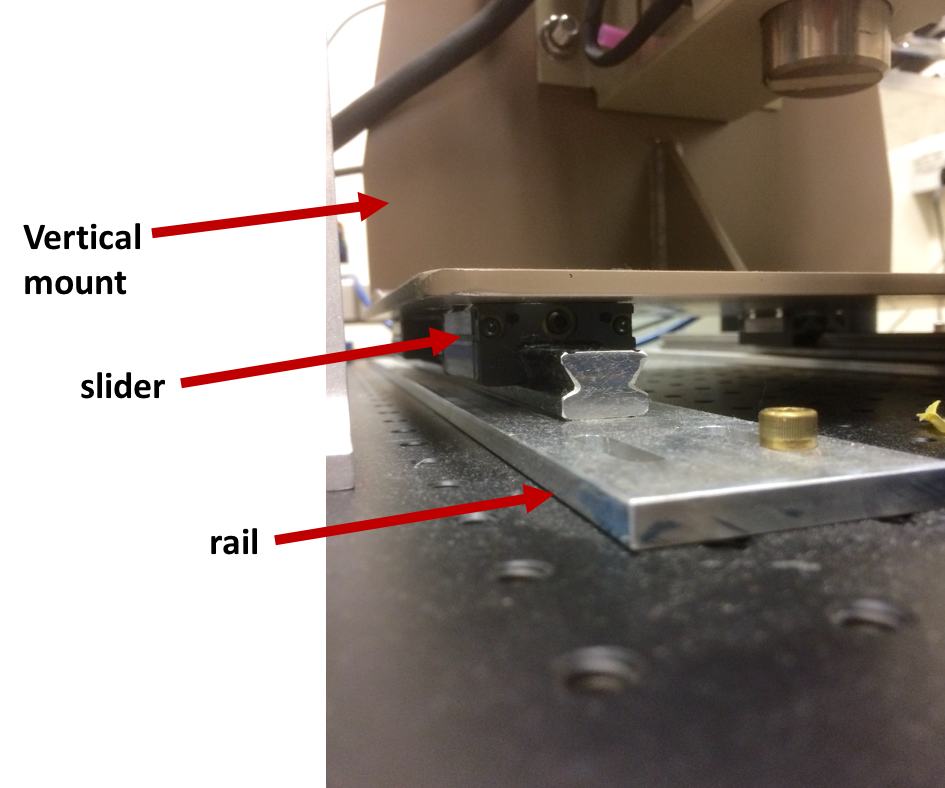
\includegraphics[width=75mm]{fig/appendix/4.png}}
\caption{(a) Side view of the magnet. (b) Bottom view of the magnet}
\end{figure}


Here is the list of equipments needed for making ST-FMR measurements up to 40 GHz.

\begin{enumerate}
  \item Signal recovery 7225 DSP lock-in Amplifier
  \item Hittite HMC-T2240 synthesized signal generator, 10 MHz to 40 GHz
  \item Clear Microwave Broadband Bias Tee BT50K40 50Khz-40GHz
  \item Keithley 2400 Source Meter (DC Source)
  \item Microwave cable : Teledyne Accutest R95-0004-072 (72 inch 1GHz- 40GHz)
  \item Pomona BNC cables

\end{enumerate}

When connecting the microwave cables, there are two small things worth notice. Firstly, all the connectors should be cleaned regularly. Secondly, the microwave cables should be supported to release all the possible tensions.

\begin{figure*}[t]
\centering
\subfigure{\label{fig:operation5}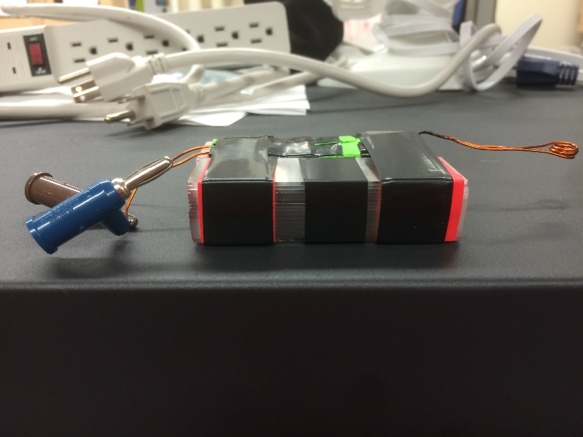
\includegraphics[width=75mm]{fig/appendix/5.png}}
\subfigure{\label{fig:operation6}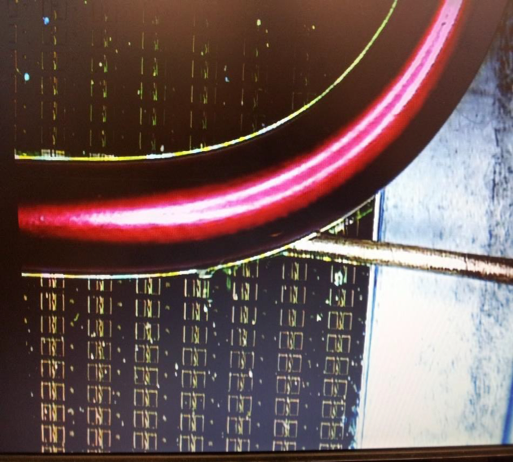
\includegraphics[width=75mm]{fig/appendix/6.png}}
\caption{(a) Coil for out-of-plane modulation (b) Wire for in-plane modulation}
\end{figure*}

The last pieces of equipments needed is the field modulation setup. Here is the list:

\begin{enumerate}
  \item Behringer EUROPOWER Professional 4,000-Watt Stereo Power Amplifier 
  \item TE CONNECTIVITY / CGS CJT10004R7JJ  Through Hole Wire wound Resistor, 4.7 Ohm
  \item High quality cable connecting from lock-in to the input of the sound amplifier : Monster Performer 500 - 10' Speaker Cable
  \item BK Precision 2831E  Ammeter to control the current through the copper wire  
\end{enumerate}
  
 When making the field-modulation coil, it is better to use any low resistance copper wire for magnetic field modulation coil. For out-of-plane field modulations, we use an external coil above the sample as shown in Fig.\ref{fig:operation5}. In-plane field modulation can be achieved by simply placing straight wire above the sample as shown in Fig.\ref{fig:operation6}. In our current design, we embed the coil into the plastic base right under the sample. It is important to ensure that the wire is not in contact with the sample or any other parts of the microwave setup. 


\begin{figure*}[h]
\centering
\subfigure{\label{fig:operation7}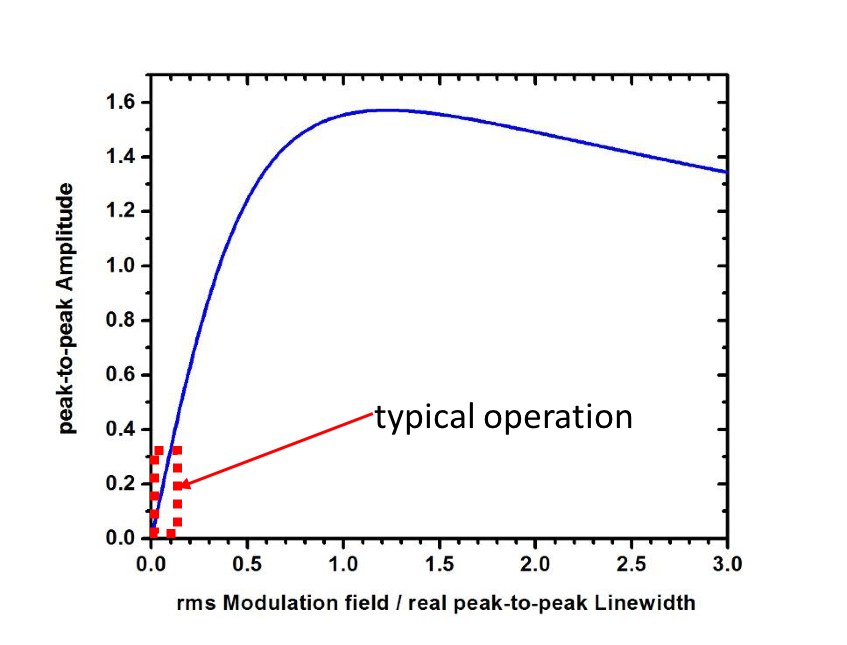
\includegraphics[width=80mm]{fig/appendix/7.png}}
\subfigure{\label{fig:operation8}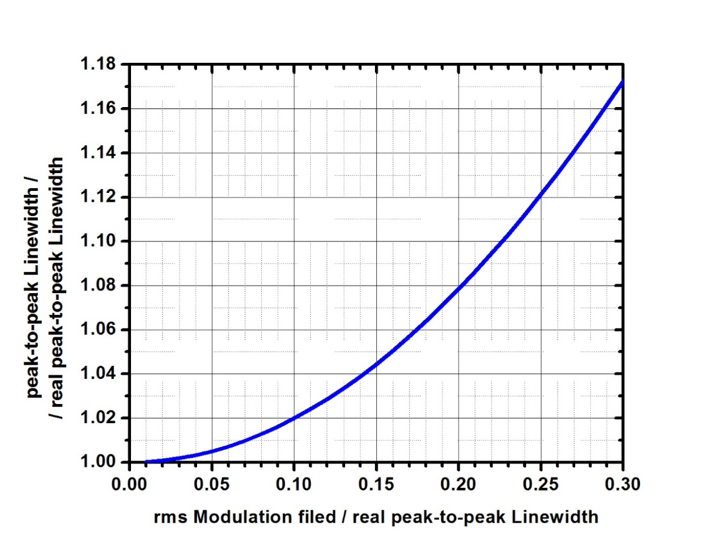
\includegraphics[width=80mm]{fig/appendix/8.png}}
\caption{(a) Peak-to-peak amplitude versus rms modulation field over real peak-to-peak linewidth. (b) peak-to-peak linewidth over real peak-to-peak linewidth versus rms modulation field over real peak-to-peak linewidth.}
\end{figure*}

In the experiment, two parameters need to be determined for the field modulation: the amplitude of modulation field and the frequency of the modulation ac field. Typically Increasing the modulation field increases the signal amplitude, but not infinitely as shown in Fig.\ref{fig:operation7}. If you are over-modulating, the signal becomes distorted and the linewidth broadens as shown in Fig.\ref{fig:operation8}. In our current setup, the input ac current is about 3.6 A to achieve the modulation field around a few oersted field, which is enough to have decent signal-to-noise ratio without distorting the spectrum.





\clearpage

\section{Best practice of ST-FMR measurement}

After connect the basic experimental and field modulation set-up, there is a few crucial steps needed for ST-FMR measurement. The first step is \textbf{External magnetic field calibration}. In our probe station, the external dc magnetic field is produced by a GMW electromagnet powering via BOP Kepco power supply. The DC current at the output 0f BOP Kepco power supplied are control by input DC voltage applied to the control input connector, which is located at the front panel of the power supply. We typically use the DAC to send the dc current into the Kepco. The following steps summarizes the field calibrations:

\begin{itemize}
  \item Place the Hall sensor of 3-axis Hall Probes(Lake Shore Cryotronics Model No.460) at the exact location of the center of magnet. This is the place we want to do the magnetic field calibration.
  \item Sweeping the DC voltage input on the Kepco power supply and recording the induced magnetic field. Typically we go from +10 volts to -10 volts. Depending the intrinsic hysteresis loop of the magnet, the field sweeping direction might affect the magnetic field value. For better precision, we record both field sweep up and sweep down data.
  \item After obtaining the data of magnetic field value as a function of applying dc voltage, we can fit the data using a five-order polynomial function(more than enough). Fig.\ref{fig:fieldcal} shows an example of field calibrations. Once this step is done, we will be able to fix the magnetic field value by applying certain amount of dc voltage(which is only one line of code)
\end{itemize}

\begin{figure*}[t]
  \centering
  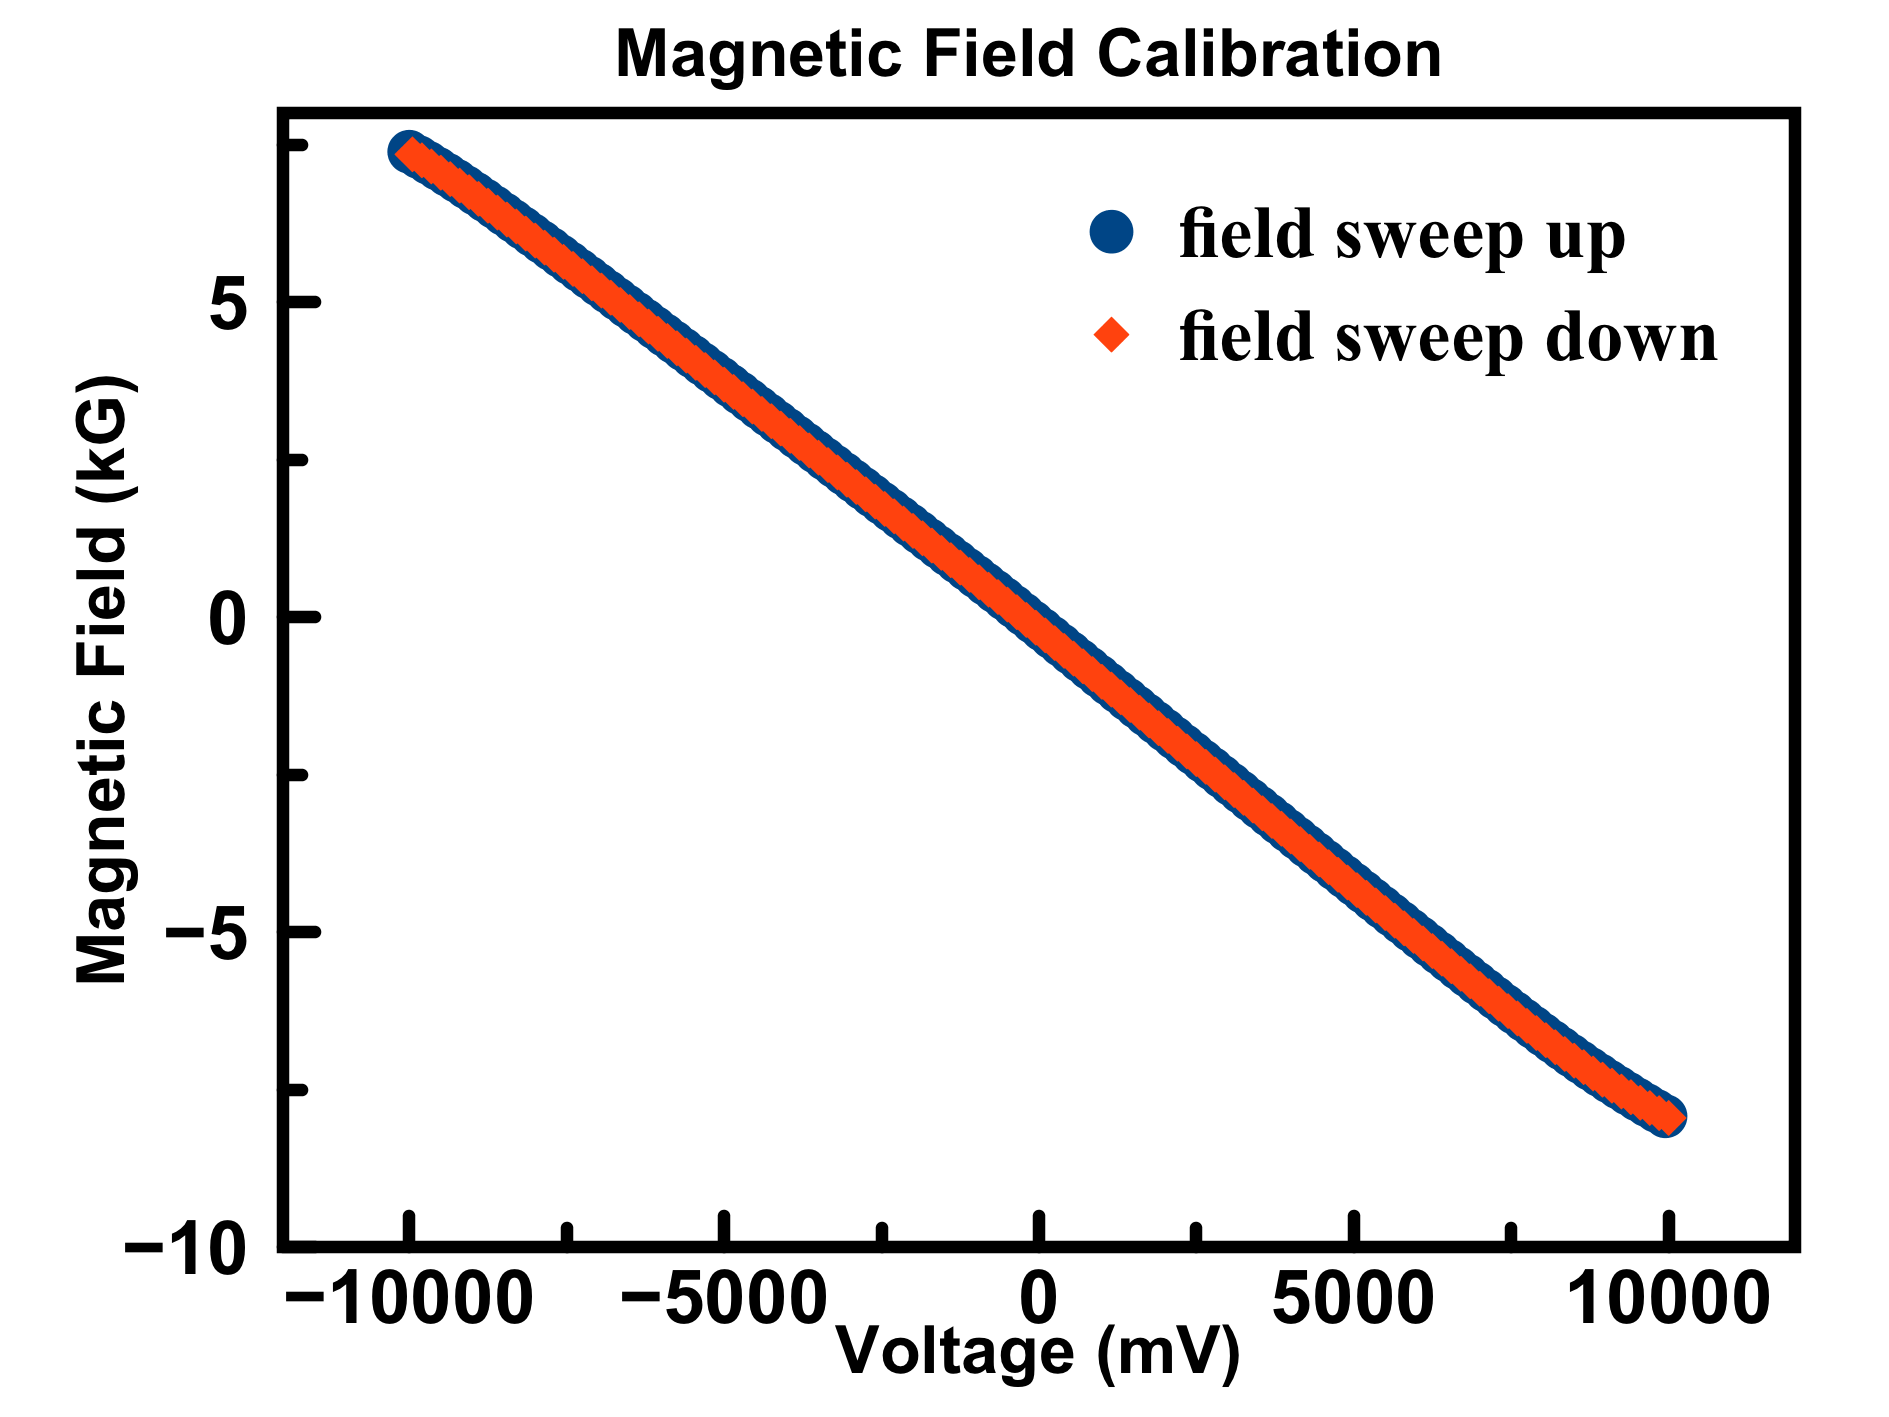
\includegraphics[width=0.8\textwidth]{fig/appendix/fieldCal.png}
  \caption{Example of field calibration}
  \label{fig:fieldcal}
\end{figure*}

The second step is \textbf{Power calibration}. When applied microwave is transmitted in the microwave cables and reflected different connectors(bias-T also), it will unavoidable power loss, which is generally frequency-dependent. In this case, if we change the applied frequency, the power at the sample would be different, which will affect the measurement result by introducing another unwanted variables. For example, both the resonance frequency and the linewidth could be altered by different microwave. In order to eliminate this unwanted variables in our measurement, we will need to perform power calibrations of each circuit used in the ST-FMR set-up. The basic steps are summarized below:
\begin{itemize}
	\item we connect the Agilent EPM Series Power Meter(model number: E4418B) with the microwave generator(with a bias Tee in between). There are two different power sensors we have in the lab. One can go up to 26.5 GHz and one can go up to 50.0 GHz. Depending on the frequency range you want, the proper power sensor is used. Also pay attention to the microwave cables used in the circuit. Many microwave cables can only go to 18 GHz. In our circuit, we only use high quality cables up to 40 GHz.
	\item Suppose we want to know the power calibration of -2 dBm at 18 GHz. We first apply -2 dBm power at 18 GHz and measure the power before the RF probe tips. The difference between -2 dBm and the measured values is the first-order power loss (P1).  Then we add the first-order power loss (P1) to -2 dBm and measure the power before the RF probe tips for the second time. Now the difference between new measured values and -2 dBm is the second-order power loss (P2). Combing the first and the second order power loss, we have updated the power loss value at this 18 GHz. Usually second-order power loss is enough for the precision requirement. By repeating this process for different frequencies, we have the final power calibrations. Ideally, you will have do power calibration for each power level you use in the real experiment.
	\item However, when going to higher frequencies(above 26 GHz), the maximum power level of the power sensor is -20 dBm, which is not the value we are likely to use in the ST-FMR measurement.  So for higher frequency power calibration, we can only obtain the real second order power loss at -20 dBm and use this value for the other power level. 
\end{itemize}

Fig.\ref{fig:powercal} shows an example of power calibration result at -20 dBm original power applied. It plots the power loss as a function of frequencies. For this plot we can see that from 5 GHz to 20 GHz, the power loss is almost linear and when going above 20 GHz, it shows a strong oscillations. Moreover, it can be seen from the plot that from 5 GHz to 20 GHz, the power loss almost increase 10 dBm, which shows the importance of power calibrations. One thing to notice that, we perform the power calibration at a 50 ohm load power meter. The resistances of real devices are much higher so the the real power at the device might be different even after power calibration. A rule of thumb of good power calibration is that when applying the magnetic field in the saturated easy axis direction, the field dispersion relation should be quite linear without any wiggles.


\begin{figure*}[h]
  \centering
  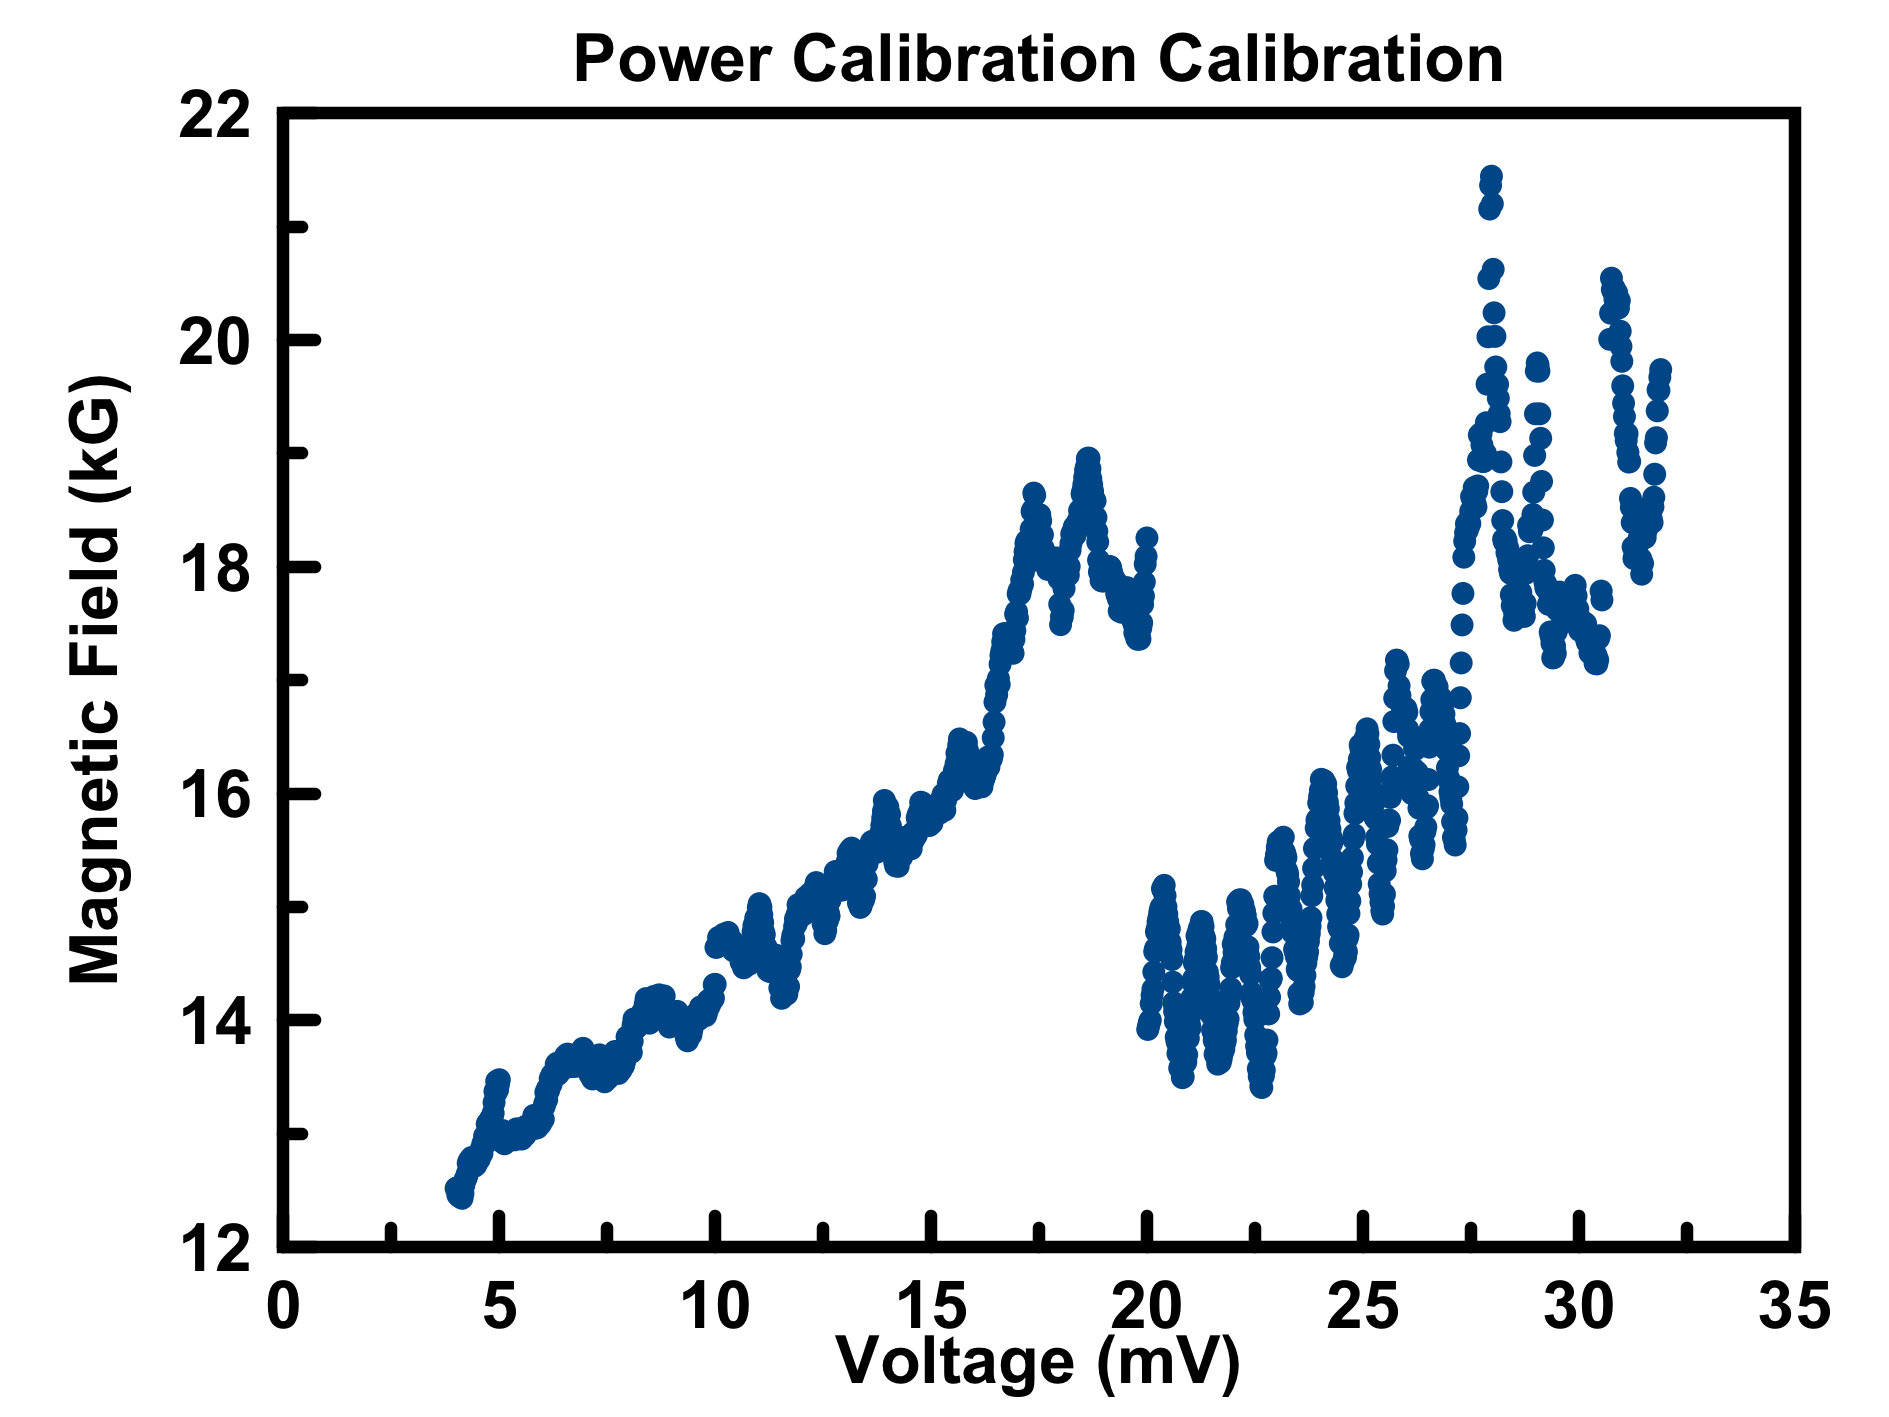
\includegraphics[width=0.8\textwidth]{fig/appendix/powerCal.png}
  \caption{Example of power calibration at -20 dBm power applied}
  \label{fig:powercal}
\end{figure*}

Now we are ready to perform the measurement. The first step(quite often) is \textbf{probe landing}. The probe operations should be practiced without over-travel(which will damage the probe) or less-travel(which will have unstable contact). After the probe has landed, we can gently knock the station table to see if the resistance of the device changes. If the resistance of the device is stable, we can then move away the microscope and slide in the perpendicular magnet. If this device is measured at the very first time, we first perform the \textbf{Resistance versus Field} measurement to obtain the magnetoresistance of this device. At the same time, we can also make sure that we have good contact of the probe. Keep in mind that if the contact is bad, the ST-FMR signal would not be good.

A few \textbf{lock-in amplifier settings} needs to be adjusted before the ST-FMR measurement. While it is true that different devices will have different optimal settings, for most of the  MTJ devices, I tend to use similar sets of settings. The following settings are used in the \textbf{Stanford Research Systems Model SR830 Lock-In Amplifier}:

\begin{itemize}
	\item \textbf{Time Constant}. Typically using \textbf{30 ms} and \textbf{24 dB}. The time constant depends on the sweeping time of each trace. You might want to use smaller time constant in case you find the trace sweeps too fast.
	\item \textbf{FET} versus \textbf{Bipolar}. These two transistors are both used in the lock-in amplifier. In short, Bipolar transistors are for low input and output impedance and FET transistors are for high input and output impedance. A more thorough comparison can be found in the Fig.\ref{fig:transistor}. For the MTJ devices, I typically find the Bipolar setting is better but the difference is quite small.
	\item \textbf{Modulation Frequency}. If considering the common $1/f$ noise in the circuit, then using higher modulation frequency is better. In fact, some of our group members try using modulation frequency 19999 Hz and get good results. However, typically I find the frequency from 987 Hz to 4003 Hz works better for MTJ devices.
	\item \textbf{Sensitivity}. In our ST-FMR measurement, there will always be some background signal. When setting the sensitivity, it is preferred to use the lowest value so that the background signal does not overload. For example, if the background signal is around 0.2 mV, then 1 mV sensitivity should be used.
	\item \textbf{Phase}. In our ST-FMR measurement, the phase setting in the lock-in amplifier does not have a strong physical meaning. We adjust the phase so that all the ST-FMR signal is in one channel and the other channel is basically flat. This can be done by \textbf{Auto Phase} options in the lock-in amplifier. 
\end{itemize}

\begin{figure*}[h]
  \centering
  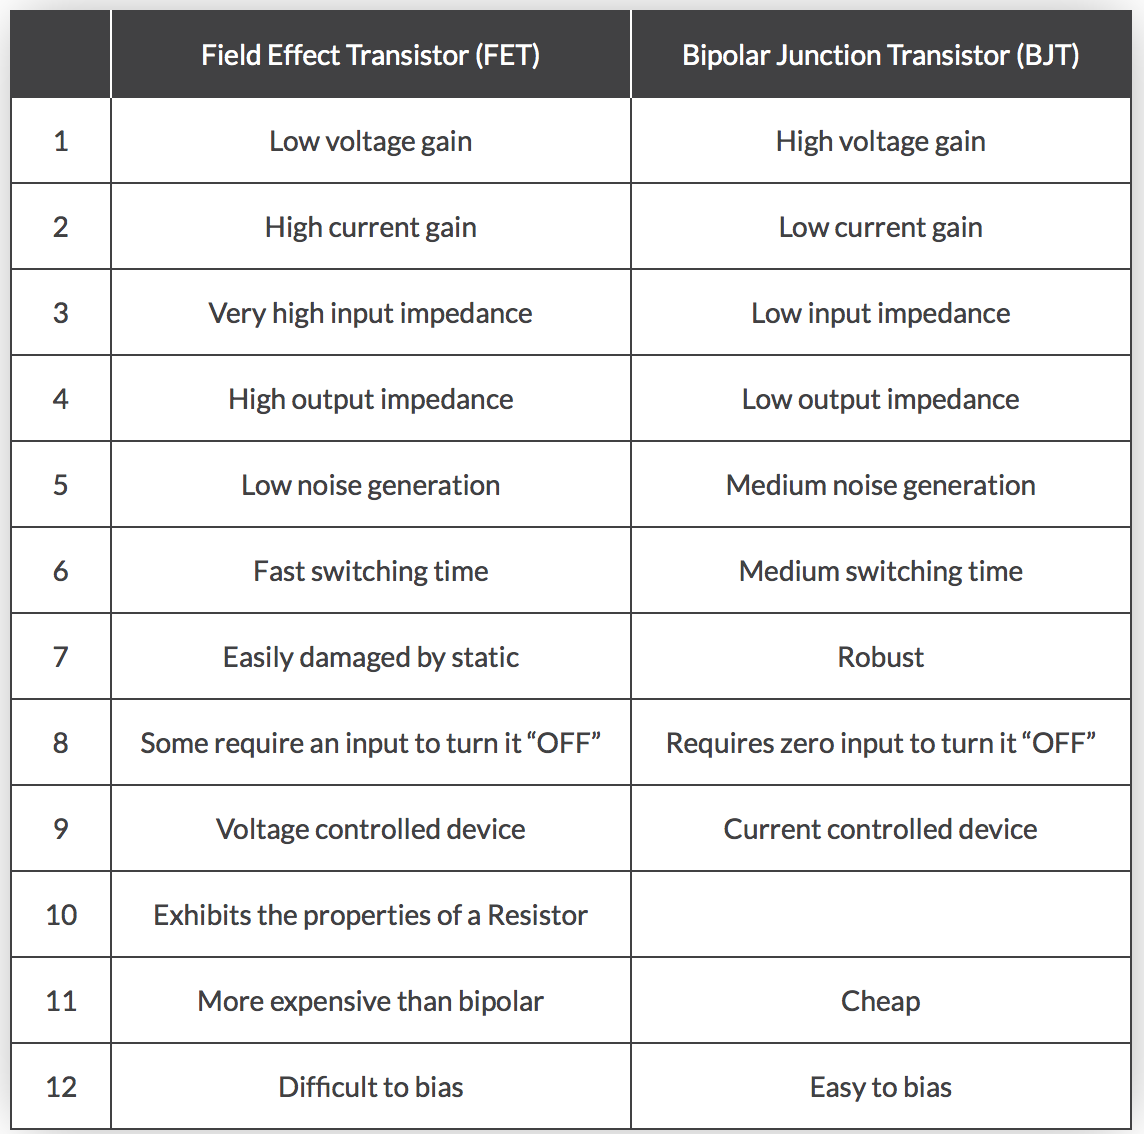
\includegraphics[width=0.8\textwidth]{fig/appendix/transistor.png}
  \caption{Difference between FET and Bipolar transistors\cite{Transistor}.}
  \label{fig:transistor}
\end{figure*}

When all the lock-in settings are done, we are ready to make the ST-FMR measurement. Whenever starting at a new device, to search for the signal. It is suggested that higher frequency(around 15 GHz)and wider magnetic field range(from -3 kG to 3 kG) should be used. Once identifying the ST-FMR signal, first varying the frequency to see if the signal shifts with magnetic field(not some measurement artifacts). Then narrowing the field range to cover all the spin wave modes. Varying the microwave power so that the signal can be boosted without distorting the spectrum(You can plot the resonance field as a function of power). Tuning all the parameters of the lock-in amplifier as listed before to get the best signal-to-noise ratio.

In our lab, all the measurement scripts are coded in \textbf{Python}, which enables easy implementations and maintenance with better add-on functionalities. All the instruments and data recordings are done within the Python scripts. We currently have developed a master version of Python scripts which contains all the basic measurements, which can be found in our group internal server. All the scripts have been tested and ready to go.

After the measurement, all the experimental data are processed using the \textbf{MagicPlot} software. Compared with \textbf{Origin}, \textbf{MagicPlot} has a much more modern user-interface with better functions, which allows for batch processing and user-defined fitting functions.

%%% Local Variables: ***
%%% mode: latex ***
%%% TeX-master: "thesis.tex" ***
%%% End: ***
